\section{The Doppler Effect \footnote{A Doppler Shift Speed Gun, Reid Sherman, Kavli Institute for Cosmological Physics, Department of Astronomy and Astrophysics, University of Chicago. Portions of this material may have been modified locally and may not have been classroom tested}}

\begin{comment}
This lab is more of a worksheet than it is a lab.  But I've used versions of if in my 132 classes for a while, so I thought it was time to include it here in the lab manual for others as well.  --Matt Trawick, 6/2015

\end{comment}

\makelabheader %(Space for student name, etc., defined in master.tex)

\vspace{0.1in}
%\textbf{Objective} 
%

\textbf{Apparatus} 

\begin{itemize}
	\item Stopwatch
	\item Meter stick
	\item Sound sensor
	\item Buzzing ball
	\item Strings to attach the buzzing ball
\end{itemize}
\vspace{0.3cm}

\textbf{Introduction}

What will happen to a sound wave when emitted by a moving object? Most of us have experienced the Doppler effect, probably in a situation where a car or motorcycle passes us at a relatively high speed. The sound, specifically the pitch or frequency, of the engine changes as the vehicle passes us. The vehicle begins by approaching us, but after it has passed, it is receding from us. This characteristic rise in frequency as the vehicle approaches and fall in frequency as the vehicle recedes is called the Doppler effect.  The Doppler effect occurs any time either the source, the observer or both are in motion.  In this lab, we're going to study the Doppler effect using a moving source; the moving observer version is similar.
\vspace{0.3cm}

\textbf{Activity 1}

Let’s think a bit more about why waves appear different if things are moving about. Imagine you are a lifeguard in a rowboat a bit off shore guarding all the swimmers at the beach, and that there are some waves evenly spaced apart, moving directly towards the beach. Every few seconds, your rowboat is rocked by a wave. 

(a) What would happen if you started to row away from the beach, toward the incoming waves? Would the waves rock your boat more or less frequently? 
\answerspace{32mm}


(b) What if you were done working and you were rowing in toward shore? 
\answerspace{32mm}

This is the essence of the Doppler effect: that waves will be more frequent if you are moving towards them or if the source of the waves is moving towards you, and they will seem less frequent if the source and the observer are moving apart.
\vspace{0.3cm}

\textbf{Activity 2: Moving Source, Fixed Receiver}

Pay attention to the demo that your instruction will perform! Your instructor will twirl a buzzing ball around their head. Also, have two partners listening from two directions and see if they hear the pitch change in the same way and at the same time.

(a) What do you hear? What do they hear? Describe how the sound changes. Is the pitch/frequency constant? The volume? Give it a try! Twirl the buzzer assembly around your head, with your partners standing several feet away. Try to swing it at a constant rate. Try to swing it at a few different speeds. Record your observations. Make sure the person swinging in the middle has a chance to be on the outside and observe the sound change.
\answerspace{30mm}

(b) How would you determine the speed of the buzzer as is it swung around? What do we need to measure? How would you measure it? (Hint: Remember circular motion from PHYS 131?)
\answerspace{30mm}

(c) Calculate the Speed of the buzzer, use 10 compete cycles. Repeat the procedure three times and find the average speed. Show your calculations in your lab notebook and record the results in a data table.
\answerspace{30mm}

Mathematically, the Doppler shift that you observed may be described by the following equations:

Source moving towards you: $f’$ observed frequency

\begin{equation}
f’ =\frac{f}{[1 - (v/v_{s})]}
\end{equation}

Source moving away from you: $f’$ observed frequency

\begin{equation}
	f’ =\frac{f}{[1 + (v/v_{s})]}
\end{equation}

where $f =$ source frequency in Hertz (Hz), $f’ =$ perceived frequency (Hz), $v =$ speed of source
and $v_{s} =$ speed of sound. The speed of sound depends on the weather (both the temperature and the humidity), but for our purposes we will assume that the speed of sound is $v_{s} = 350$ m/s.

(d) Calculate the expected perceived frequency of your buzzer by using the equations above and the average speed from your earlier measurements. What is the calculated perceived frequency when the buzzer is moving towards and away from you?
\answerspace{30mm}

(e) The human ear can hear sounds ranging from 20 Hz to 20,000 Hz. It is most sensitive to frequencies between 500 and 4,000 Hz and can distinguish between sounds that are a few Hertz different. Should a human with normal hearing be able to detect the frequency shift you calculated?
\answerspace{30mm}

\textbf{Activity 3: Measuring and comparing}

(a) Using the sound analysis software, we will now record the buzzer both at rest and while swinging it at constant speed. The software will be able to measure both the intensity and frequency of sound waves. Can you tell from the spectrum when the ball was moving towards the detector and when it was moving away?
\answerspace{32mm}

(b) What is the frequency shift?
\answerspace{32mm}

(c) Compare the measured Doppler shift to the calculated one.  Do they agree?
\answerspace{32mm}


\pagebreak
\textbf{Activity 4: Moving Source and Moving Receiver}

\begin{center}
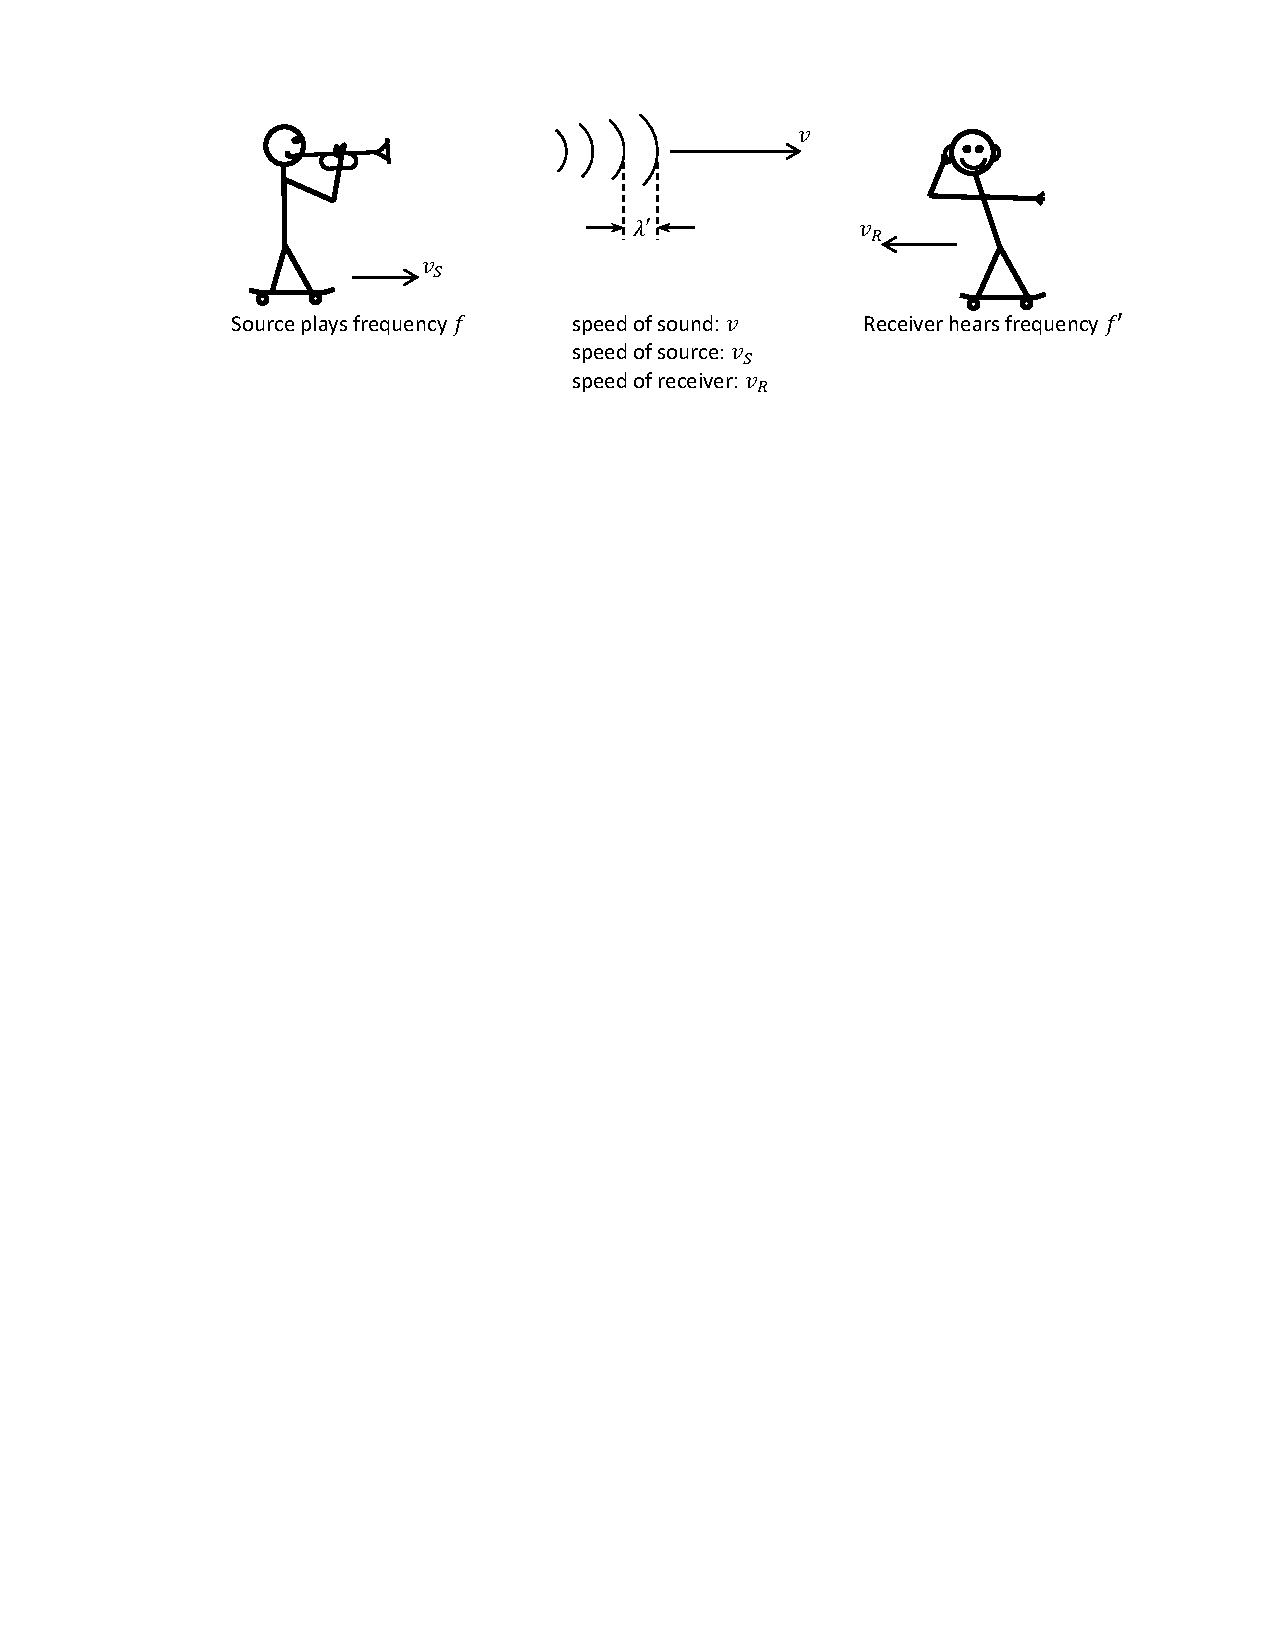
\includegraphics[width=0.75\textwidth]{doppler_shift_mariama/moving_observer.pdf}
\end{center}

Your friend (the ``source'') is playing the trumpet while riding towards you on a skateboard at speed $v_S$.  The first wavefront is emitted at time $t=0$. Now suppose that you are also moving towards the source with speed $v_R$.  

(a) What is the speed of the wave \textit{relative to the receiver}?  (That is, in the receiver reference frame, how fast do you see the wave coming at you?) 
\answerspace{30mm}

(b) What is the time $T'$ between the receiver hitting the first wavefront and the receiver hitting the second wavefront? (Answer in $\lambda', v, v_R$.)
\answerspace{30mm}

(c) Rewrite $T'$ in terms of $v, v_R, v_S$, and $f$, using your result from part (c).
\answerspace{30mm}

(d) So what frequency $f'$ does the receiver hear?
%\vspace{1.0in}

\vfill

Note our sign convention here:
\begin{align*}
\textrm{positive } v_R, v_S &\Longrightarrow \textrm{motion towards each other (``approaching'')} \\
\textrm{negative } v_R, v_S &\Longrightarrow \textrm{motion away from each other (``receding'')} 
\end{align*}


